\documentclass[1p]{elsarticle_modified}
%\bibliographystyle{elsarticle-num}

%\usepackage[colorlinks]{hyperref}
%\usepackage{abbrmath_seonhwa} %\Abb, \Ascr, \Acal ,\Abf, \Afrak
\usepackage{amsfonts}
\usepackage{amssymb}
\usepackage{amsmath}
\usepackage{amsthm}
\usepackage{scalefnt}
\usepackage{amsbsy}
\usepackage{kotex}
\usepackage{caption}
\usepackage{subfig}
\usepackage{color}
\usepackage{graphicx}
\usepackage{xcolor} %% white, black, red, green, blue, cyan, magenta, yellow
\usepackage{float}
\usepackage{setspace}
\usepackage{hyperref}

\usepackage{tikz}
\usetikzlibrary{arrows}

\usepackage{multirow}
\usepackage{array} % fixed length table
\usepackage{hhline}

%%%%%%%%%%%%%%%%%%%%%
\makeatletter
\renewcommand*\env@matrix[1][\arraystretch]{%
	\edef\arraystretch{#1}%
	\hskip -\arraycolsep
	\let\@ifnextchar\new@ifnextchar
	\array{*\c@MaxMatrixCols c}}
\makeatother %https://tex.stackexchange.com/questions/14071/how-can-i-increase-the-line-spacing-in-a-matrix
%%%%%%%%%%%%%%%

\usepackage[normalem]{ulem}

\newcommand{\msout}[1]{\ifmmode\text{\sout{\ensuremath{#1}}}\else\sout{#1}\fi}
%SOURCE: \msout is \stkout macro in https://tex.stackexchange.com/questions/20609/strikeout-in-math-mode

\newcommand{\cancel}[1]{
	\ifmmode
	{\color{red}\msout{#1}}
	\else
	{\color{red}\sout{#1}}
	\fi
}

\newcommand{\add}[1]{
	{\color{blue}\uwave{#1}}
}

\newcommand{\replace}[2]{
	\ifmmode
	{\color{red}\msout{#1}}{\color{blue}\uwave{#2}}
	\else
	{\color{red}\sout{#1}}{\color{blue}\uwave{#2}}
	\fi
}

\newcommand{\Sol}{\mathcal{S}} %segment
\newcommand{\D}{D} %diagram
\newcommand{\A}{\mathcal{A}} %arc


%%%%%%%%%%%%%%%%%%%%%%%%%%%%%5 test

\def\sl{\operatorname{\textup{SL}}(2,\Cbb)}
\def\psl{\operatorname{\textup{PSL}}(2,\Cbb)}
\def\quan{\mkern 1mu \triangleright \mkern 1mu}

\theoremstyle{definition}
\newtheorem{thm}{Theorem}[section]
\newtheorem{prop}[thm]{Proposition}
\newtheorem{lem}[thm]{Lemma}
\newtheorem{ques}[thm]{Question}
\newtheorem{cor}[thm]{Corollary}
\newtheorem{defn}[thm]{Definition}
\newtheorem{exam}[thm]{Example}
\newtheorem{rmk}[thm]{Remark}
\newtheorem{alg}[thm]{Algorithm}

\newcommand{\I}{\sqrt{-1}}
\begin{document}

%\begin{frontmatter}
%
%\title{Boundary parabolic representations of knots up to 8 crossings}
%
%%% Group authors per affiliation:
%\author{Yunhi Cho} 
%\address{Department of Mathematics, University of Seoul, Seoul, Korea}
%\ead{yhcho@uos.ac.kr}
%
%
%\author{Seonhwa Kim} %\fnref{s_kim}}
%\address{Center for Geometry and Physics, Institute for Basic Science, Pohang, 37673, Korea}
%\ead{ryeona17@ibs.re.kr}
%
%\author{Hyuk Kim}
%\address{Department of Mathematical Sciences, Seoul National University, Seoul 08826, Korea}
%\ead{hyukkim@snu.ac.kr}
%
%\author{Seokbeom Yoon}
%\address{Department of Mathematical Sciences, Seoul National University, Seoul, 08826,  Korea}
%\ead{sbyoon15@snu.ac.kr}
%
%\begin{abstract}
%We find all boundary parabolic representation of knots up to 8 crossings.
%
%\end{abstract}
%\begin{keyword}
%    \MSC[2010] 57M25 
%\end{keyword}
%
%\end{frontmatter}

%\linenumbers
%\tableofcontents
%
\newcommand\colored[1]{\textcolor{white}{\rule[-0.35ex]{0.8em}{1.4ex}}\kern-0.8em\color{red} #1}%
%\newcommand\colored[1]{\textcolor{white}{ #1}\kern-2.17ex	\textcolor{white}{ #1}\kern-1.81ex	\textcolor{white}{ #1}\kern-2.15ex\color{red}#1	}

{\Large $\underline{12a_{0909}~(K12a_{0909})}$}

\setlength{\tabcolsep}{10pt}
\renewcommand{\arraystretch}{1.6}
\vspace{1cm}\begin{tabular}{m{100pt}>{\centering\arraybackslash}m{274pt}}
\multirow{5}{120pt}{
	\centering
	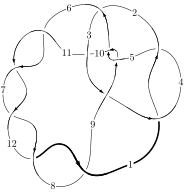
\includegraphics[width=112pt]{../../../GIT/diagram.site/Diagrams/png/1710_12a_0909.png}\\
\ \ \ A knot diagram\footnotemark}&
\allowdisplaybreaks
\textbf{Linearized knot diagam} \\
\cline{2-2}
 &
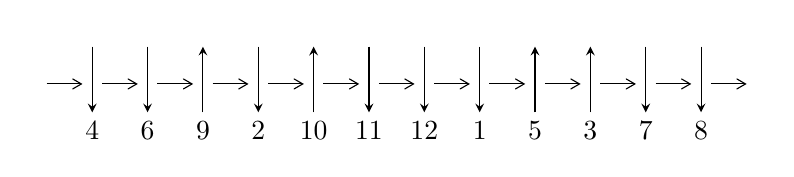
\begin{tikzpicture}[x=20pt, y=17pt]
	% nodes
	\node (C0) at (0, 0) {};
	\node (C1) at (1, 0) {};
	\node (C1U) at (1, +1) {};
	\node (C1D) at (1, -1) {4};

	\node (C2) at (2, 0) {};
	\node (C2U) at (2, +1) {};
	\node (C2D) at (2, -1) {6};

	\node (C3) at (3, 0) {};
	\node (C3U) at (3, +1) {};
	\node (C3D) at (3, -1) {9};

	\node (C4) at (4, 0) {};
	\node (C4U) at (4, +1) {};
	\node (C4D) at (4, -1) {2};

	\node (C5) at (5, 0) {};
	\node (C5U) at (5, +1) {};
	\node (C5D) at (5, -1) {10};

	\node (C6) at (6, 0) {};
	\node (C6U) at (6, +1) {};
	\node (C6D) at (6, -1) {11};

	\node (C7) at (7, 0) {};
	\node (C7U) at (7, +1) {};
	\node (C7D) at (7, -1) {12};

	\node (C8) at (8, 0) {};
	\node (C8U) at (8, +1) {};
	\node (C8D) at (8, -1) {1};

	\node (C9) at (9, 0) {};
	\node (C9U) at (9, +1) {};
	\node (C9D) at (9, -1) {5};

	\node (C10) at (10, 0) {};
	\node (C10U) at (10, +1) {};
	\node (C10D) at (10, -1) {3};

	\node (C11) at (11, 0) {};
	\node (C11U) at (11, +1) {};
	\node (C11D) at (11, -1) {7};

	\node (C12) at (12, 0) {};
	\node (C12U) at (12, +1) {};
	\node (C12D) at (12, -1) {8};
	\node (C13) at (13, 0) {};

	% arrows
	\draw[->,>={angle 60}]
	(C0) edge (C1) (C1) edge (C2) (C2) edge (C3) (C3) edge (C4) (C4) edge (C5) (C5) edge (C6) (C6) edge (C7) (C7) edge (C8) (C8) edge (C9) (C9) edge (C10) (C10) edge (C11) (C11) edge (C12) (C12) edge (C13) ;	\draw[->,>=stealth]
	(C1U) edge (C1D) (C2U) edge (C2D) (C3D) edge (C3U) (C4U) edge (C4D) (C5D) edge (C5U) (C6U) edge (C6D) (C7U) edge (C7D) (C8U) edge (C8D) (C9D) edge (C9U) (C10D) edge (C10U) (C11U) edge (C11D) (C12U) edge (C12D) ;
	\end{tikzpicture} \\
\hhline{~~} \\& 
\textbf{Solving Sequence} \\ \cline{2-2} 
 &
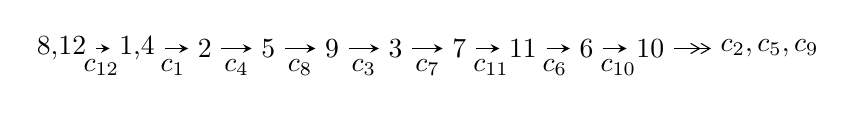
\begin{tikzpicture}[x=23pt, y=7pt]
	% node
	\node (A0) at (-1/8, 0) {8,12};
	\node (A1) at (17/16, 0) {1,4};
	\node (A2) at (17/8, 0) {2};
	\node (A3) at (25/8, 0) {5};
	\node (A4) at (33/8, 0) {9};
	\node (A5) at (41/8, 0) {3};
	\node (A6) at (49/8, 0) {7};
	\node (A7) at (57/8, 0) {11};
	\node (A8) at (65/8, 0) {6};
	\node (A9) at (73/8, 0) {10};
	\node (C1) at (1/2, -1) {$c_{12}$};
	\node (C2) at (13/8, -1) {$c_{1}$};
	\node (C3) at (21/8, -1) {$c_{4}$};
	\node (C4) at (29/8, -1) {$c_{8}$};
	\node (C5) at (37/8, -1) {$c_{3}$};
	\node (C6) at (45/8, -1) {$c_{7}$};
	\node (C7) at (53/8, -1) {$c_{11}$};
	\node (C8) at (61/8, -1) {$c_{6}$};
	\node (C9) at (69/8, -1) {$c_{10}$};
	\node (A10) at (11, 0) {$c_{2},c_{5},c_{9}$};

	% edge
	\draw[->,>=stealth]	
	(A0) edge (A1) (A1) edge (A2) (A2) edge (A3) (A3) edge (A4) (A4) edge (A5) (A5) edge (A6) (A6) edge (A7) (A7) edge (A8) (A8) edge (A9) ;
	\draw[->>,>={angle 60}]	
	(A9) edge (A10);
\end{tikzpicture} \\ 

\end{tabular} \\

\footnotetext{
The image of knot diagram is generated by the software ``\textbf{Draw programme}" developed by Andrew Bartholomew(\url{http://www.layer8.co.uk/maths/draw/index.htm\#Running-draw}), where we modified some parts for our purpose(\url{https://github.com/CATsTAILs/LinksPainter}).
}\phantom \\ \newline 
\centering \textbf{Ideals for irreducible components\footnotemark of $X_{\text{par}}$} 
 
\begin{align*}
I^u_{1}&=\langle 
-2.13178\times10^{29} u^{50}+5.14130\times10^{28} u^{49}+\cdots+1.65837\times10^{29} b-2.15608\times10^{27},\\
\phantom{I^u_{1}}&\phantom{= \langle  }-1.15795\times10^{29} u^{50}+4.35679\times10^{28} u^{49}+\cdots+1.65837\times10^{29} a+6.77432\times10^{28},\;u^{51}-2 u^{50}+\cdots- u+1\rangle \\
I^u_{2}&=\langle 
b-1,\;a-1,\;u+1\rangle \\
\\
\end{align*}
\raggedright * 2 irreducible components of $\dim_{\mathbb{C}}=0$, with total 52 representations.\\
\footnotetext{All coefficients of polynomials are rational numbers. But the coefficients are sometimes approximated in decimal forms when there is not enough margin.}
\newpage
\renewcommand{\arraystretch}{1}
\centering \section*{I. $I^u_{1}= \langle -2.13\times10^{29} u^{50}+5.14\times10^{28} u^{49}+\cdots+1.66\times10^{29} b-2.16\times10^{27},\;-1.16\times10^{29} u^{50}+4.36\times10^{28} u^{49}+\cdots+1.66\times10^{29} a+6.77\times10^{28},\;u^{51}-2 u^{50}+\cdots- u+1 \rangle$}
\flushleft \textbf{(i) Arc colorings}\\
\begin{tabular}{m{7pt} m{180pt} m{7pt} m{180pt} }
\flushright $a_{8}=$&$\begin{pmatrix}0\\u\end{pmatrix}$ \\
\flushright $a_{12}=$&$\begin{pmatrix}1\\0\end{pmatrix}$ \\
\flushright $a_{1}=$&$\begin{pmatrix}1\\u^2\end{pmatrix}$ \\
\flushright $a_{4}=$&$\begin{pmatrix}0.698249 u^{50}-0.262716 u^{49}+\cdots-11.7227 u-0.408493\\1.28547 u^{50}-0.310022 u^{49}+\cdots+0.0538566 u+0.0130012\end{pmatrix}$ \\
\flushright $a_{2}=$&$\begin{pmatrix}0.674876 u^{50}-0.229531 u^{49}+\cdots-12.1488 u+0.603479\\1.22229 u^{50}-0.317787 u^{49}+\cdots+0.264395 u+0.0354543\end{pmatrix}$ \\
\flushright $a_{5}=$&$\begin{pmatrix}0.137080 u^{50}+0.0189458 u^{49}+\cdots+0.718302 u-1.06415\\0.412183 u^{50}+0.00870488 u^{49}+\cdots-0.371603 u-0.128201\end{pmatrix}$ \\
\flushright $a_{9}=$&$\begin{pmatrix}- u\\- u^3+u\end{pmatrix}$ \\
\flushright $a_{3}=$&$\begin{pmatrix}-0.568625 u^{50}+0.203922 u^{49}+\cdots-12.2253 u+0.626397\\-1.07781 u^{50}+0.232253 u^{49}+\cdots-0.243835 u+1.04522\end{pmatrix}$ \\
\flushright $a_{7}=$&$\begin{pmatrix}u\\u\end{pmatrix}$ \\
\flushright $a_{11}=$&$\begin{pmatrix}- u^2+1\\- u^2\end{pmatrix}$ \\
\flushright $a_{6}=$&$\begin{pmatrix}- u^3+2 u\\- u^3+u\end{pmatrix}$ \\
\flushright $a_{10}=$&$\begin{pmatrix}-0.275103 u^{50}+0.0102409 u^{49}+\cdots+1.08990 u-0.935948\\-0.412183 u^{50}-0.00870488 u^{49}+\cdots+0.371603 u+0.128201\end{pmatrix}$\\&\end{tabular}
\flushleft \textbf{(ii) Obstruction class $= -1$}\\~\\
\flushleft \textbf{(iii) Cusp Shapes $= -1.08773 u^{50}+4.19995 u^{49}+\cdots-16.8202 u-2.33236$}\\~\\
\newpage\renewcommand{\arraystretch}{1}
\flushleft \textbf{(iv) u-Polynomials at the component}\newline \\
\begin{tabular}{m{50pt}|m{274pt}}
Crossings & \hspace{64pt}u-Polynomials at each crossing \\
\hline $$\begin{aligned}c_{1},c_{4}\end{aligned}$$&$\begin{aligned}
&u^{51}-3 u^{50}+\cdots-87 u+9
\end{aligned}$\\
\hline $$\begin{aligned}c_{2}\end{aligned}$$&$\begin{aligned}
&17(17 u^{51}-112 u^{50}+\cdots+151 u-17)
\end{aligned}$\\
\hline $$\begin{aligned}c_{3}\end{aligned}$$&$\begin{aligned}
&17(17 u^{51}-228 u^{50}+\cdots-4473 u+2377)
\end{aligned}$\\
\hline $$\begin{aligned}c_{5},c_{9}\end{aligned}$$&$\begin{aligned}
&u^{51}-15 u^{49}+\cdots-3 u-1
\end{aligned}$\\
\hline $$\begin{aligned}c_{6},c_{7},c_{8}\\c_{11},c_{12}\end{aligned}$$&$\begin{aligned}
&u^{51}-2 u^{50}+\cdots- u+1
\end{aligned}$\\
\hline $$\begin{aligned}c_{10}\end{aligned}$$&$\begin{aligned}
&u^{51}+3 u^{50}+\cdots-291 u-51
\end{aligned}$\\
\hline
\end{tabular}\\~\\
\newpage\renewcommand{\arraystretch}{1}
\flushleft \textbf{(v) Riley Polynomials at the component}\newline \\
\begin{tabular}{m{50pt}|m{274pt}}
Crossings & \hspace{64pt}Riley Polynomials at each crossing \\
\hline $$\begin{aligned}c_{1},c_{4}\end{aligned}$$&$\begin{aligned}
&y^{51}-39 y^{50}+\cdots+5175 y-81
\end{aligned}$\\
\hline $$\begin{aligned}c_{2}\end{aligned}$$&$\begin{aligned}
&289(289 y^{51}-39098 y^{50}+\cdots+18449 y-289)
\end{aligned}$\\
\hline $$\begin{aligned}c_{3}\end{aligned}$$&$\begin{aligned}
&289(289 y^{51}-30598 y^{50}+\cdots+2.10558\times10^{8} y-5650129)
\end{aligned}$\\
\hline $$\begin{aligned}c_{5},c_{9}\end{aligned}$$&$\begin{aligned}
&y^{51}-30 y^{50}+\cdots+9 y-1
\end{aligned}$\\
\hline $$\begin{aligned}c_{6},c_{7},c_{8}\\c_{11},c_{12}\end{aligned}$$&$\begin{aligned}
&y^{51}-70 y^{50}+\cdots+9 y-1
\end{aligned}$\\
\hline $$\begin{aligned}c_{10}\end{aligned}$$&$\begin{aligned}
&y^{51}+9 y^{50}+\cdots+43575 y-2601
\end{aligned}$\\
\hline
\end{tabular}\\~\\
\newpage\flushleft \textbf{(vi) Complex Volumes and Cusp Shapes}
$$\begin{array}{c|c|c}  
\text{Solutions to }I^u_{1}& \I (\text{vol} + \sqrt{-1}CS) & \text{Cusp shape}\\
 \hline 
\begin{aligned}
u &= \phantom{-}1.047260 + 0.151588 I \\
a &= -0.338923 + 0.162440 I \\
b &= -0.065433 + 0.787075 I\end{aligned}
 & -4.15821 - 2.51727 I & \phantom{-0.000000 } 0 \\ \hline\begin{aligned}
u &= \phantom{-}1.047260 - 0.151588 I \\
a &= -0.338923 - 0.162440 I \\
b &= -0.065433 - 0.787075 I\end{aligned}
 & -4.15821 + 2.51727 I & \phantom{-0.000000 } 0 \\ \hline\begin{aligned}
u &= -1.077900 + 0.210349 I \\
a &= -0.414562 + 0.513194 I \\
b &= -0.211649 - 0.453660 I\end{aligned}
 & -1.01874 + 6.10618 I & \phantom{-0.000000 } 0 \\ \hline\begin{aligned}
u &= -1.077900 - 0.210349 I \\
a &= -0.414562 - 0.513194 I \\
b &= -0.211649 + 0.453660 I\end{aligned}
 & -1.01874 - 6.10618 I & \phantom{-0.000000 } 0 \\ \hline\begin{aligned}
u &= -0.890510\phantom{ +0.000000I} \\
a &= \phantom{-}0.780361\phantom{ +0.000000I} \\
b &= \phantom{-}0.512763\phantom{ +0.000000I}\end{aligned}
 & -1.69978\phantom{ +0.000000I} & -4.88630\phantom{ +0.000000I} \\ \hline\begin{aligned}
u &= -1.120720 + 0.024853 I \\
a &= -2.15005 - 0.20348 I \\
b &= -1.208940 - 0.347028 I\end{aligned}
 & -6.84706 + 0.17814 I & \phantom{-0.000000 } 0 \\ \hline\begin{aligned}
u &= -1.120720 - 0.024853 I \\
a &= -2.15005 + 0.20348 I \\
b &= -1.208940 + 0.347028 I\end{aligned}
 & -6.84706 - 0.17814 I & \phantom{-0.000000 } 0 \\ \hline\begin{aligned}
u &= \phantom{-}1.126260 + 0.086381 I \\
a &= -1.61198 + 0.21718 I \\
b &= -0.738481 + 0.732354 I\end{aligned}
 & -5.85482 - 3.55367 I & \phantom{-0.000000 } 0 \\ \hline\begin{aligned}
u &= \phantom{-}1.126260 - 0.086381 I \\
a &= -1.61198 - 0.21718 I \\
b &= -0.738481 - 0.732354 I\end{aligned}
 & -5.85482 + 3.55367 I & \phantom{-0.000000 } 0 \\ \hline\begin{aligned}
u &= -0.438374 + 0.708518 I \\
a &= \phantom{-}0.366935 + 0.769343 I \\
b &= -0.844551 - 0.361467 I\end{aligned}
 & -4.09880 + 2.34673 I & -13.7642 - 6.0920 I\\
 \hline 
 \end{array}$$\newpage$$\begin{array}{c|c|c}  
\text{Solutions to }I^u_{1}& \I (\text{vol} + \sqrt{-1}CS) & \text{Cusp shape}\\
 \hline 
\begin{aligned}
u &= -0.438374 - 0.708518 I \\
a &= \phantom{-}0.366935 - 0.769343 I \\
b &= -0.844551 + 0.361467 I\end{aligned}
 & -4.09880 - 2.34673 I & -13.7642 + 6.0920 I \\ \hline\begin{aligned}
u &= -1.170700 + 0.336077 I \\
a &= \phantom{-}1.80050 + 0.84662 I \\
b &= \phantom{-}1.55082 + 0.18031 I\end{aligned}
 & -5.46811 + 12.11320 I & \phantom{-0.000000 } 0 \\ \hline\begin{aligned}
u &= -1.170700 - 0.336077 I \\
a &= \phantom{-}1.80050 - 0.84662 I \\
b &= \phantom{-}1.55082 - 0.18031 I\end{aligned}
 & -5.46811 - 12.11320 I & \phantom{-0.000000 } 0 \\ \hline\begin{aligned}
u &= -1.140670 + 0.479406 I \\
a &= \phantom{-}1.072900 + 0.758069 I \\
b &= \phantom{-}0.825477 - 0.456373 I\end{aligned}
 & -4.33250 - 0.67320 I & \phantom{-0.000000 } 0 \\ \hline\begin{aligned}
u &= -1.140670 - 0.479406 I \\
a &= \phantom{-}1.072900 - 0.758069 I \\
b &= \phantom{-}0.825477 + 0.456373 I\end{aligned}
 & -4.33250 + 0.67320 I & \phantom{-0.000000 } 0 \\ \hline\begin{aligned}
u &= \phantom{-}0.436309 + 0.619055 I \\
a &= \phantom{-}0.571431 - 1.171610 I \\
b &= -0.742635 + 0.081884 I\end{aligned}
 & -0.40580 - 8.83491 I & -5.93498 + 8.65489 I \\ \hline\begin{aligned}
u &= \phantom{-}0.436309 - 0.619055 I \\
a &= \phantom{-}0.571431 + 1.171610 I \\
b &= -0.742635 - 0.081884 I\end{aligned}
 & -0.40580 + 8.83491 I & -5.93498 - 8.65489 I \\ \hline\begin{aligned}
u &= \phantom{-}1.190350 + 0.364165 I \\
a &= \phantom{-}1.55085 - 0.82569 I \\
b &= \phantom{-}1.381760 + 0.003819 I\end{aligned}
 & -9.25343 - 5.99551 I & \phantom{-0.000000 } 0 \\ \hline\begin{aligned}
u &= \phantom{-}1.190350 - 0.364165 I \\
a &= \phantom{-}1.55085 + 0.82569 I \\
b &= \phantom{-}1.381760 - 0.003819 I\end{aligned}
 & -9.25343 + 5.99551 I & \phantom{-0.000000 } 0 \\ \hline\begin{aligned}
u &= \phantom{-}0.299142 + 0.682434 I \\
a &= -0.097433 - 0.386283 I \\
b &= -0.974446 + 0.425322 I\end{aligned}
 & \phantom{-}0.02412 + 4.64525 I & -6.01152 - 5.00660 I\\
 \hline 
 \end{array}$$\newpage$$\begin{array}{c|c|c}  
\text{Solutions to }I^u_{1}& \I (\text{vol} + \sqrt{-1}CS) & \text{Cusp shape}\\
 \hline 
\begin{aligned}
u &= \phantom{-}0.299142 - 0.682434 I \\
a &= -0.097433 + 0.386283 I \\
b &= -0.974446 - 0.425322 I\end{aligned}
 & \phantom{-}0.02412 - 4.64525 I & -6.01152 + 5.00660 I \\ \hline\begin{aligned}
u &= -1.34834\phantom{ +0.000000I} \\
a &= \phantom{-}1.42591\phantom{ +0.000000I} \\
b &= \phantom{-}1.94067\phantom{ +0.000000I}\end{aligned}
 & -2.22043\phantom{ +0.000000I} & \phantom{-0.000000 } 0 \\ \hline\begin{aligned}
u &= \phantom{-}0.380677 + 0.380330 I \\
a &= \phantom{-}1.68381 - 0.54757 I \\
b &= -0.0243995 - 0.1158830 I\end{aligned}
 & \phantom{-}3.01854 + 1.08074 I & -0.68742 + 2.46829 I \\ \hline\begin{aligned}
u &= \phantom{-}0.380677 - 0.380330 I \\
a &= \phantom{-}1.68381 + 0.54757 I \\
b &= -0.0243995 + 0.1158830 I\end{aligned}
 & \phantom{-}3.01854 - 1.08074 I & -0.68742 - 2.46829 I \\ \hline\begin{aligned}
u &= \phantom{-}0.295738 + 0.444672 I \\
a &= -0.187973 + 0.763692 I \\
b &= -0.269582 + 0.799798 I\end{aligned}
 & \phantom{-}3.28922 - 3.89695 I & -0.59685 + 7.26004 I \\ \hline\begin{aligned}
u &= \phantom{-}0.295738 - 0.444672 I \\
a &= -0.187973 - 0.763692 I \\
b &= -0.269582 - 0.799798 I\end{aligned}
 & \phantom{-}3.28922 + 3.89695 I & -0.59685 - 7.26004 I \\ \hline\begin{aligned}
u &= -0.390664 + 0.229819 I \\
a &= -0.02035 - 1.55893 I \\
b &= \phantom{-}0.805995 - 0.679439 I\end{aligned}
 & -1.04347 + 2.52944 I & -8.36979 - 8.40912 I \\ \hline\begin{aligned}
u &= -0.390664 - 0.229819 I \\
a &= -0.02035 + 1.55893 I \\
b &= \phantom{-}0.805995 + 0.679439 I\end{aligned}
 & -1.04347 - 2.52944 I & -8.36979 + 8.40912 I \\ \hline\begin{aligned}
u &= \phantom{-}0.400437\phantom{ +0.000000I} \\
a &= -0.797854\phantom{ +0.000000I} \\
b &= \phantom{-}1.13406\phantom{ +0.000000I}\end{aligned}
 & -2.10246\phantom{ +0.000000I} & -9.62010\phantom{ +0.000000I} \\ \hline\begin{aligned}
u &= -0.216099 + 0.323578 I \\
a &= \phantom{-}0.636723 - 0.775106 I \\
b &= \phantom{-}0.035450 - 0.334693 I\end{aligned}
 & -0.210137 + 0.904024 I & -4.53571 - 7.39815 I\\
 \hline 
 \end{array}$$\newpage$$\begin{array}{c|c|c}  
\text{Solutions to }I^u_{1}& \I (\text{vol} + \sqrt{-1}CS) & \text{Cusp shape}\\
 \hline 
\begin{aligned}
u &= -0.216099 - 0.323578 I \\
a &= \phantom{-}0.636723 + 0.775106 I \\
b &= \phantom{-}0.035450 + 0.334693 I\end{aligned}
 & -0.210137 - 0.904024 I & -4.53571 + 7.39815 I \\ \hline\begin{aligned}
u &= \phantom{-}0.330272\phantom{ +0.000000I} \\
a &= -1.79695\phantom{ +0.000000I} \\
b &= \phantom{-}0.951690\phantom{ +0.000000I}\end{aligned}
 & -2.13241\phantom{ +0.000000I} & -5.70430\phantom{ +0.000000I} \\ \hline\begin{aligned}
u &= -0.111190 + 0.292412 I \\
a &= \phantom{-}4.56602 - 1.68963 I \\
b &= \phantom{-}0.566891 + 0.031398 I\end{aligned}
 & -0.202413 - 0.749454 I & \phantom{-}1.38825 - 9.49663 I \\ \hline\begin{aligned}
u &= -0.111190 - 0.292412 I \\
a &= \phantom{-}4.56602 + 1.68963 I \\
b &= \phantom{-}0.566891 - 0.031398 I\end{aligned}
 & -0.202413 + 0.749454 I & \phantom{-}1.38825 + 9.49663 I \\ \hline\begin{aligned}
u &= \phantom{-}1.72101 + 0.02434 I \\
a &= \phantom{-}0.523521 + 0.113299 I \\
b &= \phantom{-}1.54117 + 0.66770 I\end{aligned}
 & -11.27570 - 0.29543 I & \phantom{-0.000000 } 0 \\ \hline\begin{aligned}
u &= \phantom{-}1.72101 - 0.02434 I \\
a &= \phantom{-}0.523521 - 0.113299 I \\
b &= \phantom{-}1.54117 - 0.66770 I\end{aligned}
 & -11.27570 + 0.29543 I & \phantom{-0.000000 } 0 \\ \hline\begin{aligned}
u &= -1.73799\phantom{ +0.000000I} \\
a &= -7.71129\phantom{ +0.000000I} \\
b &= -22.2616\phantom{ +0.000000I}\end{aligned}
 & -13.2279\phantom{ +0.000000I} & \phantom{-0.000000 } 0 \\ \hline\begin{aligned}
u &= -1.74438 + 0.03663 I \\
a &= -0.436565 + 0.244633 I \\
b &= -0.910713 - 0.160686 I\end{aligned}
 & -14.2469 + 3.2818 I & \phantom{-0.000000 } 0 \\ \hline\begin{aligned}
u &= -1.74438 - 0.03663 I \\
a &= -0.436565 - 0.244633 I \\
b &= -0.910713 + 0.160686 I\end{aligned}
 & -14.2469 - 3.2818 I & \phantom{-0.000000 } 0 \\ \hline\begin{aligned}
u &= \phantom{-}1.74976 + 0.05001 I \\
a &= -0.269790 - 0.861011 I \\
b &= -0.63067 - 1.27223 I\end{aligned}
 & -11.21760 - 7.16998 I & \phantom{-0.000000 } 0\\
 \hline 
 \end{array}$$\newpage$$\begin{array}{c|c|c}  
\text{Solutions to }I^u_{1}& \I (\text{vol} + \sqrt{-1}CS) & \text{Cusp shape}\\
 \hline 
\begin{aligned}
u &= \phantom{-}1.74976 - 0.05001 I \\
a &= -0.269790 + 0.861011 I \\
b &= -0.63067 + 1.27223 I\end{aligned}
 & -11.21760 + 7.16998 I & \phantom{-0.000000 } 0 \\ \hline\begin{aligned}
u &= \phantom{-}1.76103 + 0.00664 I \\
a &= -2.28196 + 0.03399 I \\
b &= -5.41561 + 0.35170 I\end{aligned}
 & -17.3264 - 0.3153 I & \phantom{-0.000000 } 0 \\ \hline\begin{aligned}
u &= \phantom{-}1.76103 - 0.00664 I \\
a &= -2.28196 - 0.03399 I \\
b &= -5.41561 - 0.35170 I\end{aligned}
 & -17.3264 + 0.3153 I & \phantom{-0.000000 } 0 \\ \hline\begin{aligned}
u &= -1.76201 + 0.01966 I \\
a &= -1.82088 + 0.20804 I \\
b &= -4.16074 - 0.13010 I\end{aligned}
 & -16.3513 + 3.9914 I & \phantom{-0.000000 } 0 \\ \hline\begin{aligned}
u &= -1.76201 - 0.01966 I \\
a &= -1.82088 - 0.20804 I \\
b &= -4.16074 + 0.13010 I\end{aligned}
 & -16.3513 - 3.9914 I & \phantom{-0.000000 } 0 \\ \hline\begin{aligned}
u &= \phantom{-}1.77148 + 0.08896 I \\
a &= \phantom{-}2.05324 - 0.41872 I \\
b &= \phantom{-}5.09853 - 1.25029 I\end{aligned}
 & -16.0463 - 13.9639 I & \phantom{-0.000000 } 0 \\ \hline\begin{aligned}
u &= \phantom{-}1.77148 - 0.08896 I \\
a &= \phantom{-}2.05324 + 0.41872 I \\
b &= \phantom{-}5.09853 + 1.25029 I\end{aligned}
 & -16.0463 + 13.9639 I & \phantom{-0.000000 } 0 \\ \hline\begin{aligned}
u &= -1.77662 + 0.09436 I \\
a &= \phantom{-}1.91281 + 0.46826 I \\
b &= \phantom{-}4.74582 + 1.21071 I\end{aligned}
 & \phantom{-}19.5628 + 7.9919 I & \phantom{-0.000000 } 0 \\ \hline\begin{aligned}
u &= -1.77662 - 0.09436 I \\
a &= \phantom{-}1.91281 - 0.46826 I \\
b &= \phantom{-}4.74582 - 1.21071 I\end{aligned}
 & \phantom{-}19.5628 - 7.9919 I & \phantom{-0.000000 } 0 \\ \hline\begin{aligned}
u &= \phantom{-}1.79336 + 0.11215 I \\
a &= \phantom{-}1.64752 - 0.41305 I \\
b &= \phantom{-}4.21301 - 0.77958 I\end{aligned}
 & -14.9728 - 1.9325 I & \phantom{-0.000000 } 0\\
 \hline 
 \end{array}$$\newpage$$\begin{array}{c|c|c}  
\text{Solutions to }I^u_{1}& \I (\text{vol} + \sqrt{-1}CS) & \text{Cusp shape}\\
 \hline 
\begin{aligned}
u &= \phantom{-}1.79336 - 0.11215 I \\
a &= \phantom{-}1.64752 + 0.41305 I \\
b &= \phantom{-}4.21301 + 0.77958 I\end{aligned}
 & -14.9728 + 1.9325 I & \phantom{-0.000000 } 0\\
 \hline 
 \end{array}$$\newpage\newpage\renewcommand{\arraystretch}{1}
\centering \section*{II. $I^u_{2}= \langle b-1,\;a-1,\;u+1 \rangle$}
\flushleft \textbf{(i) Arc colorings}\\
\begin{tabular}{m{7pt} m{180pt} m{7pt} m{180pt} }
\flushright $a_{8}=$&$\begin{pmatrix}0\\-1\end{pmatrix}$ \\
\flushright $a_{12}=$&$\begin{pmatrix}1\\0\end{pmatrix}$ \\
\flushright $a_{1}=$&$\begin{pmatrix}1\\1\end{pmatrix}$ \\
\flushright $a_{4}=$&$\begin{pmatrix}1\\1\end{pmatrix}$ \\
\flushright $a_{2}=$&$\begin{pmatrix}1\\1\end{pmatrix}$ \\
\flushright $a_{5}=$&$\begin{pmatrix}1\\1\end{pmatrix}$ \\
\flushright $a_{9}=$&$\begin{pmatrix}1\\0\end{pmatrix}$ \\
\flushright $a_{3}=$&$\begin{pmatrix}0\\1\end{pmatrix}$ \\
\flushright $a_{7}=$&$\begin{pmatrix}-1\\-1\end{pmatrix}$ \\
\flushright $a_{11}=$&$\begin{pmatrix}0\\-1\end{pmatrix}$ \\
\flushright $a_{6}=$&$\begin{pmatrix}-1\\0\end{pmatrix}$ \\
\flushright $a_{10}=$&$\begin{pmatrix}0\\-1\end{pmatrix}$\\&\end{tabular}
\flushleft \textbf{(ii) Obstruction class $= -1$}\\~\\
\flushleft \textbf{(iii) Cusp Shapes $= -6$}\\~\\
\newpage\renewcommand{\arraystretch}{1}
\flushleft \textbf{(iv) u-Polynomials at the component}\newline \\
\begin{tabular}{m{50pt}|m{274pt}}
Crossings & \hspace{64pt}u-Polynomials at each crossing \\
\hline $$\begin{aligned}c_{1},c_{4},c_{10}\end{aligned}$$&$\begin{aligned}
&u
\end{aligned}$\\
\hline $$\begin{aligned}c_{2}\end{aligned}$$&$\begin{aligned}
&u-1
\end{aligned}$\\
\hline $$\begin{aligned}c_{3},c_{5},c_{6}\\c_{7},c_{8},c_{9}\\c_{11},c_{12}\end{aligned}$$&$\begin{aligned}
&u+1
\end{aligned}$\\
\hline
\end{tabular}\\~\\
\newpage\renewcommand{\arraystretch}{1}
\flushleft \textbf{(v) Riley Polynomials at the component}\newline \\
\begin{tabular}{m{50pt}|m{274pt}}
Crossings & \hspace{64pt}Riley Polynomials at each crossing \\
\hline $$\begin{aligned}c_{1},c_{4},c_{10}\end{aligned}$$&$\begin{aligned}
&y
\end{aligned}$\\
\hline $$\begin{aligned}c_{2},c_{3},c_{5}\\c_{6},c_{7},c_{8}\\c_{9},c_{11},c_{12}\end{aligned}$$&$\begin{aligned}
&y-1
\end{aligned}$\\
\hline
\end{tabular}\\~\\
\newpage\flushleft \textbf{(vi) Complex Volumes and Cusp Shapes}
$$\begin{array}{c|c|c}  
\text{Solutions to }I^u_{2}& \I (\text{vol} + \sqrt{-1}CS) & \text{Cusp shape}\\
 \hline 
\begin{aligned}
u &= -1.00000\phantom{ +0.000000I} \\
a &= \phantom{-}1.00000\phantom{ +0.000000I} \\
b &= \phantom{-}1.00000\phantom{ +0.000000I}\end{aligned}
 & -1.64493\phantom{ +0.000000I} & -6.00000\phantom{ +0.000000I}\\
 \hline 
 \end{array}$$\newpage
\newpage\renewcommand{\arraystretch}{1}
\centering \section*{ III. u-Polynomials}
\begin{tabular}{m{50pt}|m{274pt}}
Crossings & \hspace{64pt}u-Polynomials at each crossing \\
\hline $$\begin{aligned}c_{1},c_{4}\end{aligned}$$&$\begin{aligned}
&u(u^{51}-3 u^{50}+\cdots-87 u+9)
\end{aligned}$\\
\hline $$\begin{aligned}c_{2}\end{aligned}$$&$\begin{aligned}
&17(u-1)(17 u^{51}-112 u^{50}+\cdots+151 u-17)
\end{aligned}$\\
\hline $$\begin{aligned}c_{3}\end{aligned}$$&$\begin{aligned}
&17(u+1)(17 u^{51}-228 u^{50}+\cdots-4473 u+2377)
\end{aligned}$\\
\hline $$\begin{aligned}c_{5},c_{9}\end{aligned}$$&$\begin{aligned}
&(u+1)(u^{51}-15 u^{49}+\cdots-3 u-1)
\end{aligned}$\\
\hline $$\begin{aligned}c_{6},c_{7},c_{8}\\c_{11},c_{12}\end{aligned}$$&$\begin{aligned}
&(u+1)(u^{51}-2 u^{50}+\cdots- u+1)
\end{aligned}$\\
\hline $$\begin{aligned}c_{10}\end{aligned}$$&$\begin{aligned}
&u(u^{51}+3 u^{50}+\cdots-291 u-51)
\end{aligned}$\\
\hline
\end{tabular}\newpage\renewcommand{\arraystretch}{1}
\centering \section*{ IV. Riley Polynomials}
\begin{tabular}{m{50pt}|m{274pt}}
Crossings & \hspace{64pt}Riley Polynomials at each crossing \\
\hline $$\begin{aligned}c_{1},c_{4}\end{aligned}$$&$\begin{aligned}
&y(y^{51}-39 y^{50}+\cdots+5175 y-81)
\end{aligned}$\\
\hline $$\begin{aligned}c_{2}\end{aligned}$$&$\begin{aligned}
&289(y-1)(289 y^{51}-39098 y^{50}+\cdots+18449 y-289)
\end{aligned}$\\
\hline $$\begin{aligned}c_{3}\end{aligned}$$&$\begin{aligned}
&289(y-1)(289 y^{51}-30598 y^{50}+\cdots+2.10558\times10^{8} y-5650129)
\end{aligned}$\\
\hline $$\begin{aligned}c_{5},c_{9}\end{aligned}$$&$\begin{aligned}
&(y-1)(y^{51}-30 y^{50}+\cdots+9 y-1)
\end{aligned}$\\
\hline $$\begin{aligned}c_{6},c_{7},c_{8}\\c_{11},c_{12}\end{aligned}$$&$\begin{aligned}
&(y-1)(y^{51}-70 y^{50}+\cdots+9 y-1)
\end{aligned}$\\
\hline $$\begin{aligned}c_{10}\end{aligned}$$&$\begin{aligned}
&y(y^{51}+9 y^{50}+\cdots+43575 y-2601)
\end{aligned}$\\
\hline
\end{tabular}
\vskip 2pc
\end{document}